\section{Inference}

Our trained model performs SAR to optical image translation through a two-stage inference pipeline that combines the power of latent diffusion with conditional generation capabilities.

\subsection{Inference Methodology}

\subsubsection{Input Preprocessing}

The inference process begins with preprocessing both the SAR image input and the text prompt:

\textbf{SAR Image Processing}:
The input SAR image undergoes normalization from the range [0,1] to [-1,1] to match the training data distribution. The image is then resized to 256×256×3 dimensions and converted to a batch tensor format for processing.

\textbf{Text Prompt Encoding}:
Text prompts follow the standardized format used during training: "Colorise image, Region: \{region\}, Season: \{season\}". The CLIP text encoder processes these prompts to generate 512-dimensional embeddings that capture semantic information about the geographic and temporal context.

\subsubsection{Latent Generation Process}

The core of our inference pipeline employs Denoising Diffusion Probabilistic Model (DDPM)\cite{ho2020denoisingdiffusionprobabilisticmodels} sampling with classifier-free guidance:

\begin{enumerate}
    \item \textbf{Noise Initialization}: Random Gaussian noise is initialized in the latent space with dimensions (1, 4, 64, 64)
    \item \textbf{Iterative Denoising}: The process iterates through 1000 timesteps in reverse order
    \item \textbf{Conditional Prediction}: At each timestep, the U-Net predicts noise conditioned on both the SAR image and text embedding
    \item \textbf{Classifier-Free Guidance}: The model applies guidance scaling (Gamma = 7.5) to balance conditioning fidelity and output diversity
    \item \textbf{Latent Refinement}: The scheduler updates the latent representation by removing predicted noise
\end{enumerate}

The guidance mechanism combines conditional and unconditional predictions using the formula:
\begin{equation}
\epsilon_{guided} = \epsilon_{uncond} + \gamma \cdot (\epsilon_{cond} - \epsilon_{uncond})
\end{equation}

where $\gamma = 7.5$ represents the guidance scale that balances conditioning strength and generation diversity.

\subsubsection{Image Reconstruction}

The final stage involves decoding the clean latents back to RGB image space:

\begin{enumerate}
    \item \textbf{VAE Decoding}: The trained VAE decoder transforms latents (64×64×4) to full-resolution images (256×256×3)
    \item \textbf{Post-processing}: Output values are rescaled from [-1,1] to [0,1] and clamped to ensure valid pixel ranges
    \item \textbf{Format Conversion}: The final tensor is converted to standard image format for visualization or further processing
\end{enumerate}

\subsection{Sample Results}

Our model demonstrates strong capability in generating realistic optical images from SAR inputs across various geographic regions and seasonal conditions. 

\begin{figure}[h!]
    \centering
    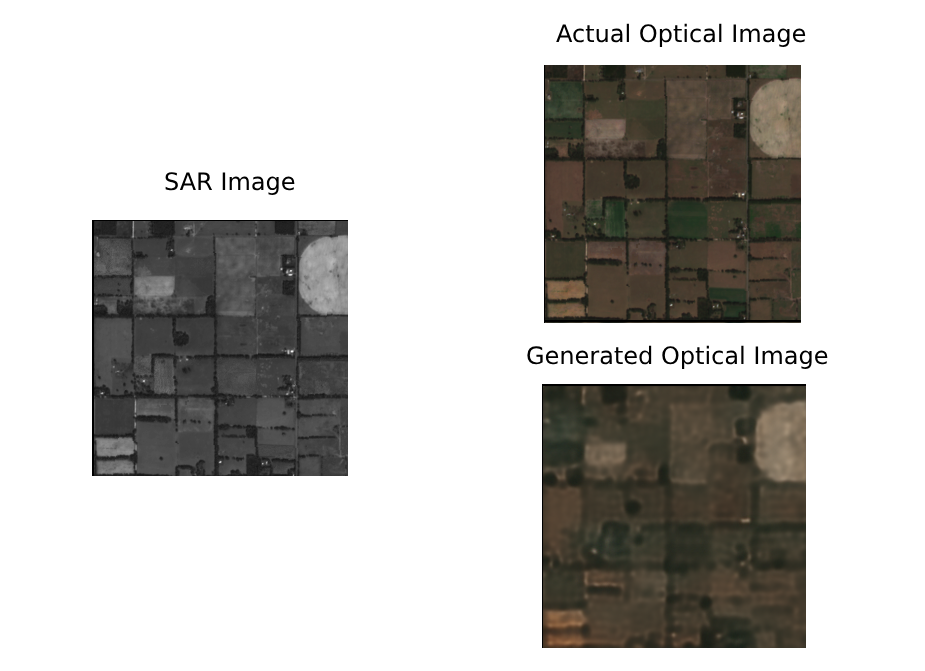
\includegraphics[width=0.8\textwidth]{sample_output_1.png}
    \caption{Sample SAR to optical translation result}
    \label{fig:sample_output_1}
\end{figure}

\begin{figure}[h!]
    \centering
    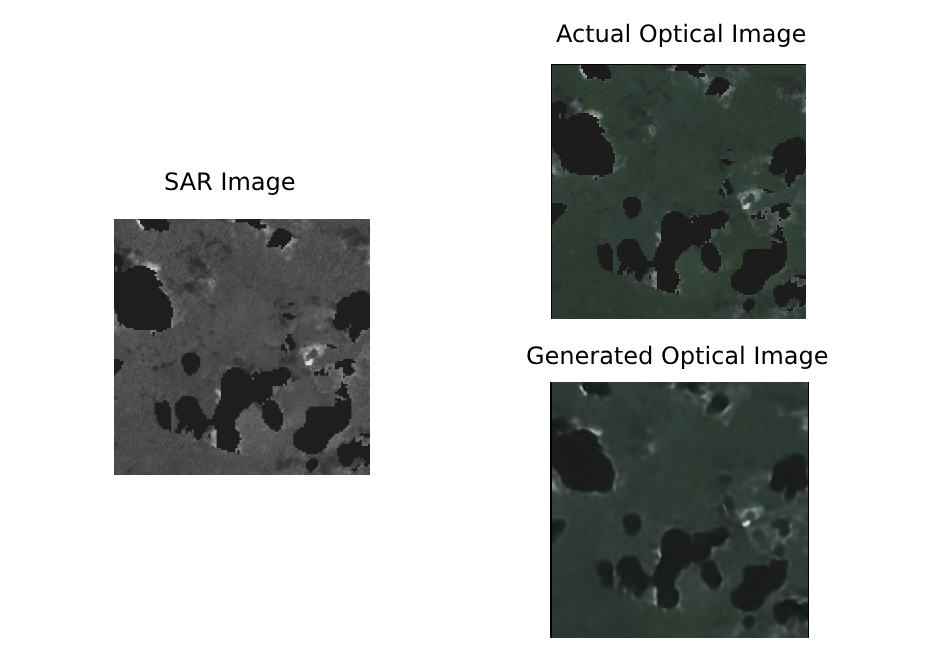
\includegraphics[width=0.8\textwidth]{sample_output_2.png}
    \caption{Additional example}
    \label{fig:sample_output_2}
\end{figure}

The generated images exhibit several key characteristics:
\begin{itemize}
    \item \textbf{Spatial Consistency}: Generated optical images maintain the spatial structure and geometric features present in the input SAR data
    \item \textbf{Contextual Appropriateness}: Colors and textures align with the specified geographic region and seasonal context
    \item \textbf{Detail Preservation}: Fine-grained features such as roads, water bodies, and vegetation boundaries are accurately preserved
    \item \textbf{Natural Appearance}: The output images exhibit realistic color distributions and visual characteristics typical of satellite optical imagery
\end{itemize}

\subsection{Web Interface}

To facilitate practical usage and demonstration of our SAR colorization system, we developed an intuitive web-based interface that allows users to upload SAR images and specify geographic and temporal parameters for generation.

\begin{figure}[h!]
    \centering
    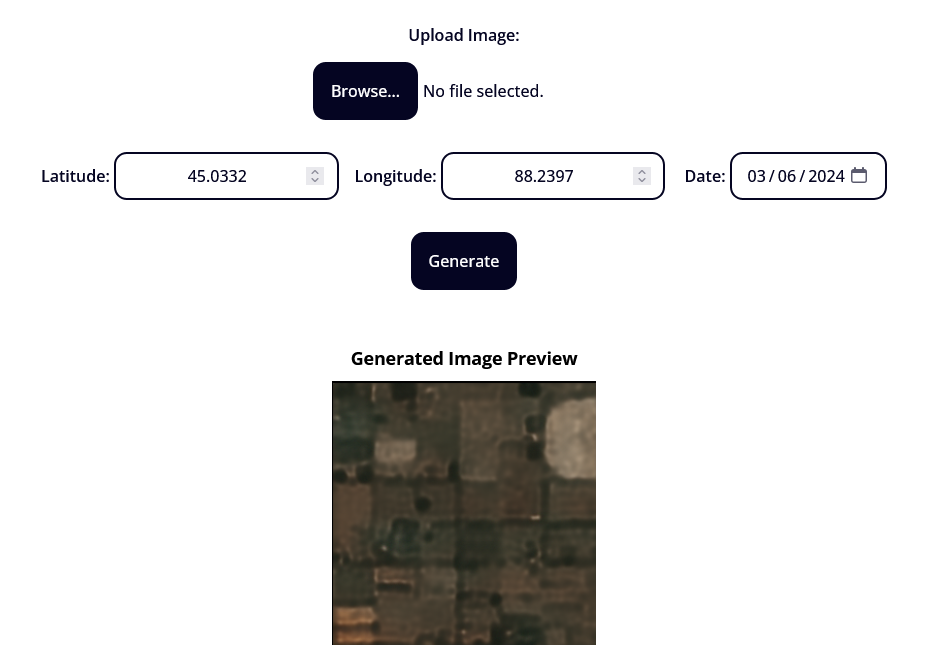
\includegraphics[width=0.8\textwidth]{web_ui.png}
    \caption{Web interface for SAR image colorization showing input controls and generated output preview}
    \label{fig:web_ui}
\end{figure}

The interface provides:
\begin{itemize}
    \item \textbf{Image Upload}: Simple drag-and-drop functionality for SAR image input
    \item \textbf{Geographic Parameters}: Latitude and longitude specification for regional context
    \item \textbf{Temporal Settings}: Date selection to determine seasonal characteristics
    \item \textbf{Real-time Preview}: Immediate visualization of generated optical imagery
\end{itemize}

\section{Evaluation}

\subsection{Evaluation Metrics}

We employ a comprehensive set of quantitative metrics to assess the quality and fidelity of our SAR to optical image translation:

\subsubsection{Peak Signal-to-Noise Ratio (PSNR)}

PSNR measures pixel-level reconstruction accuracy between generated and ground truth optical images:
\begin{equation}
PSNR = 20 \times \log_{10}\left(\frac{MAX_I}{\sqrt{MSE}}\right)
\end{equation}

where $MAX_I$ represents the maximum possible pixel value and $MSE$ is the mean squared error between images.

\subsubsection{Structural Similarity Index (SSIM)}

SSIM evaluates structural and perceptual similarity by considering luminance, contrast, and structural components:
\begin{equation}
SSIM(x,y) = \frac{(2\mu_x\mu_y + c_1)(2\sigma_{xy} + c_2)}{(\mu_x^2 + \mu_y^2 + c_1)(\sigma_x^2 + \sigma_y^2 + c_2)}
\end{equation}

SSIM values range from 0 to 1, with higher values indicating better structural preservation.

\subsubsection{Additional Metrics}

\textbf{Mean Squared Error (MSE)}:
\begin{equation}
MSE = \frac{1}{N} \sum_{i=1}^{N} (y_i - \hat{y}_i)^2
\end{equation}

\textbf{Mean Absolute Error (MAE)}:
\begin{equation}
MAE = \frac{1}{N} \sum_{i=1}^{N} |y_i - \hat{y}_i|
\end{equation}

\subsection{Experimental Results}

Our evaluation was conducted on a test dataset comprising 10 carefully selected SAR-optical image pairs representing diverse geographic regions and seasonal conditions. The model was configured with a guidance scale of 7.5 during inference to balance conditioning strength and output diversity.

\begin{table}[h!]
\centering
\begin{tabular}{|l|c|c|c|c|c|}
\hline
\textbf{Metric} & \textbf{Mean} & \textbf{Std} & \textbf{Median} & \textbf{Min} & \textbf{Max} \\
\hline
PSNR (dB) & 9.42 & 3.78 & 9.92 & 4.52 & 15.30 \\
SSIM & 0.250 & 0.172 & 0.172 & 0.107 & 0.672 \\
MSE & 0.160 & 0.119 & 0.103 & 0.030 & 0.353 \\
MAE & 0.301 & 0.142 & 0.264 & 0.121 & 0.533 \\
\hline
\end{tabular}
\caption{Quantitative evaluation results on test dataset (10 samples)}
\label{tab:evaluation_results}
\end{table}

\subsection{Performance Analysis}

\subsubsection{PSNR Analysis}
The PSNR results show a mean value of 9.42 dB with a standard deviation of 3.78 dB. While this indicates room for improvement in pixel-level accuracy, the variation in scores (4.52 to 15.30 dB) suggests that performance varies significantly across different types of terrain and imaging conditions. The relatively low PSNR values are typical for cross-modal translation tasks where exact pixel matching is less meaningful than structural and semantic correspondence.

\subsubsection{SSIM Performance}
The SSIM scores demonstrate a mean of 0.250, indicating moderate structural similarity between generated and ground truth images. The high standard deviation (0.172) and wide range (0.107 to 0.672) suggest that the model performs better on certain types of landscapes than others. The maximum SSIM of 0.672 indicates that for some samples, the model achieves good structural preservation.

\subsubsection{Error Metrics}
Both MSE (mean: 0.160) and MAE (mean: 0.301) values indicate the average magnitude of differences between generated and reference images. The relatively high standard deviations suggest significant variation in reconstruction quality across different samples.

\begin{figure}[h!]
    \centering
    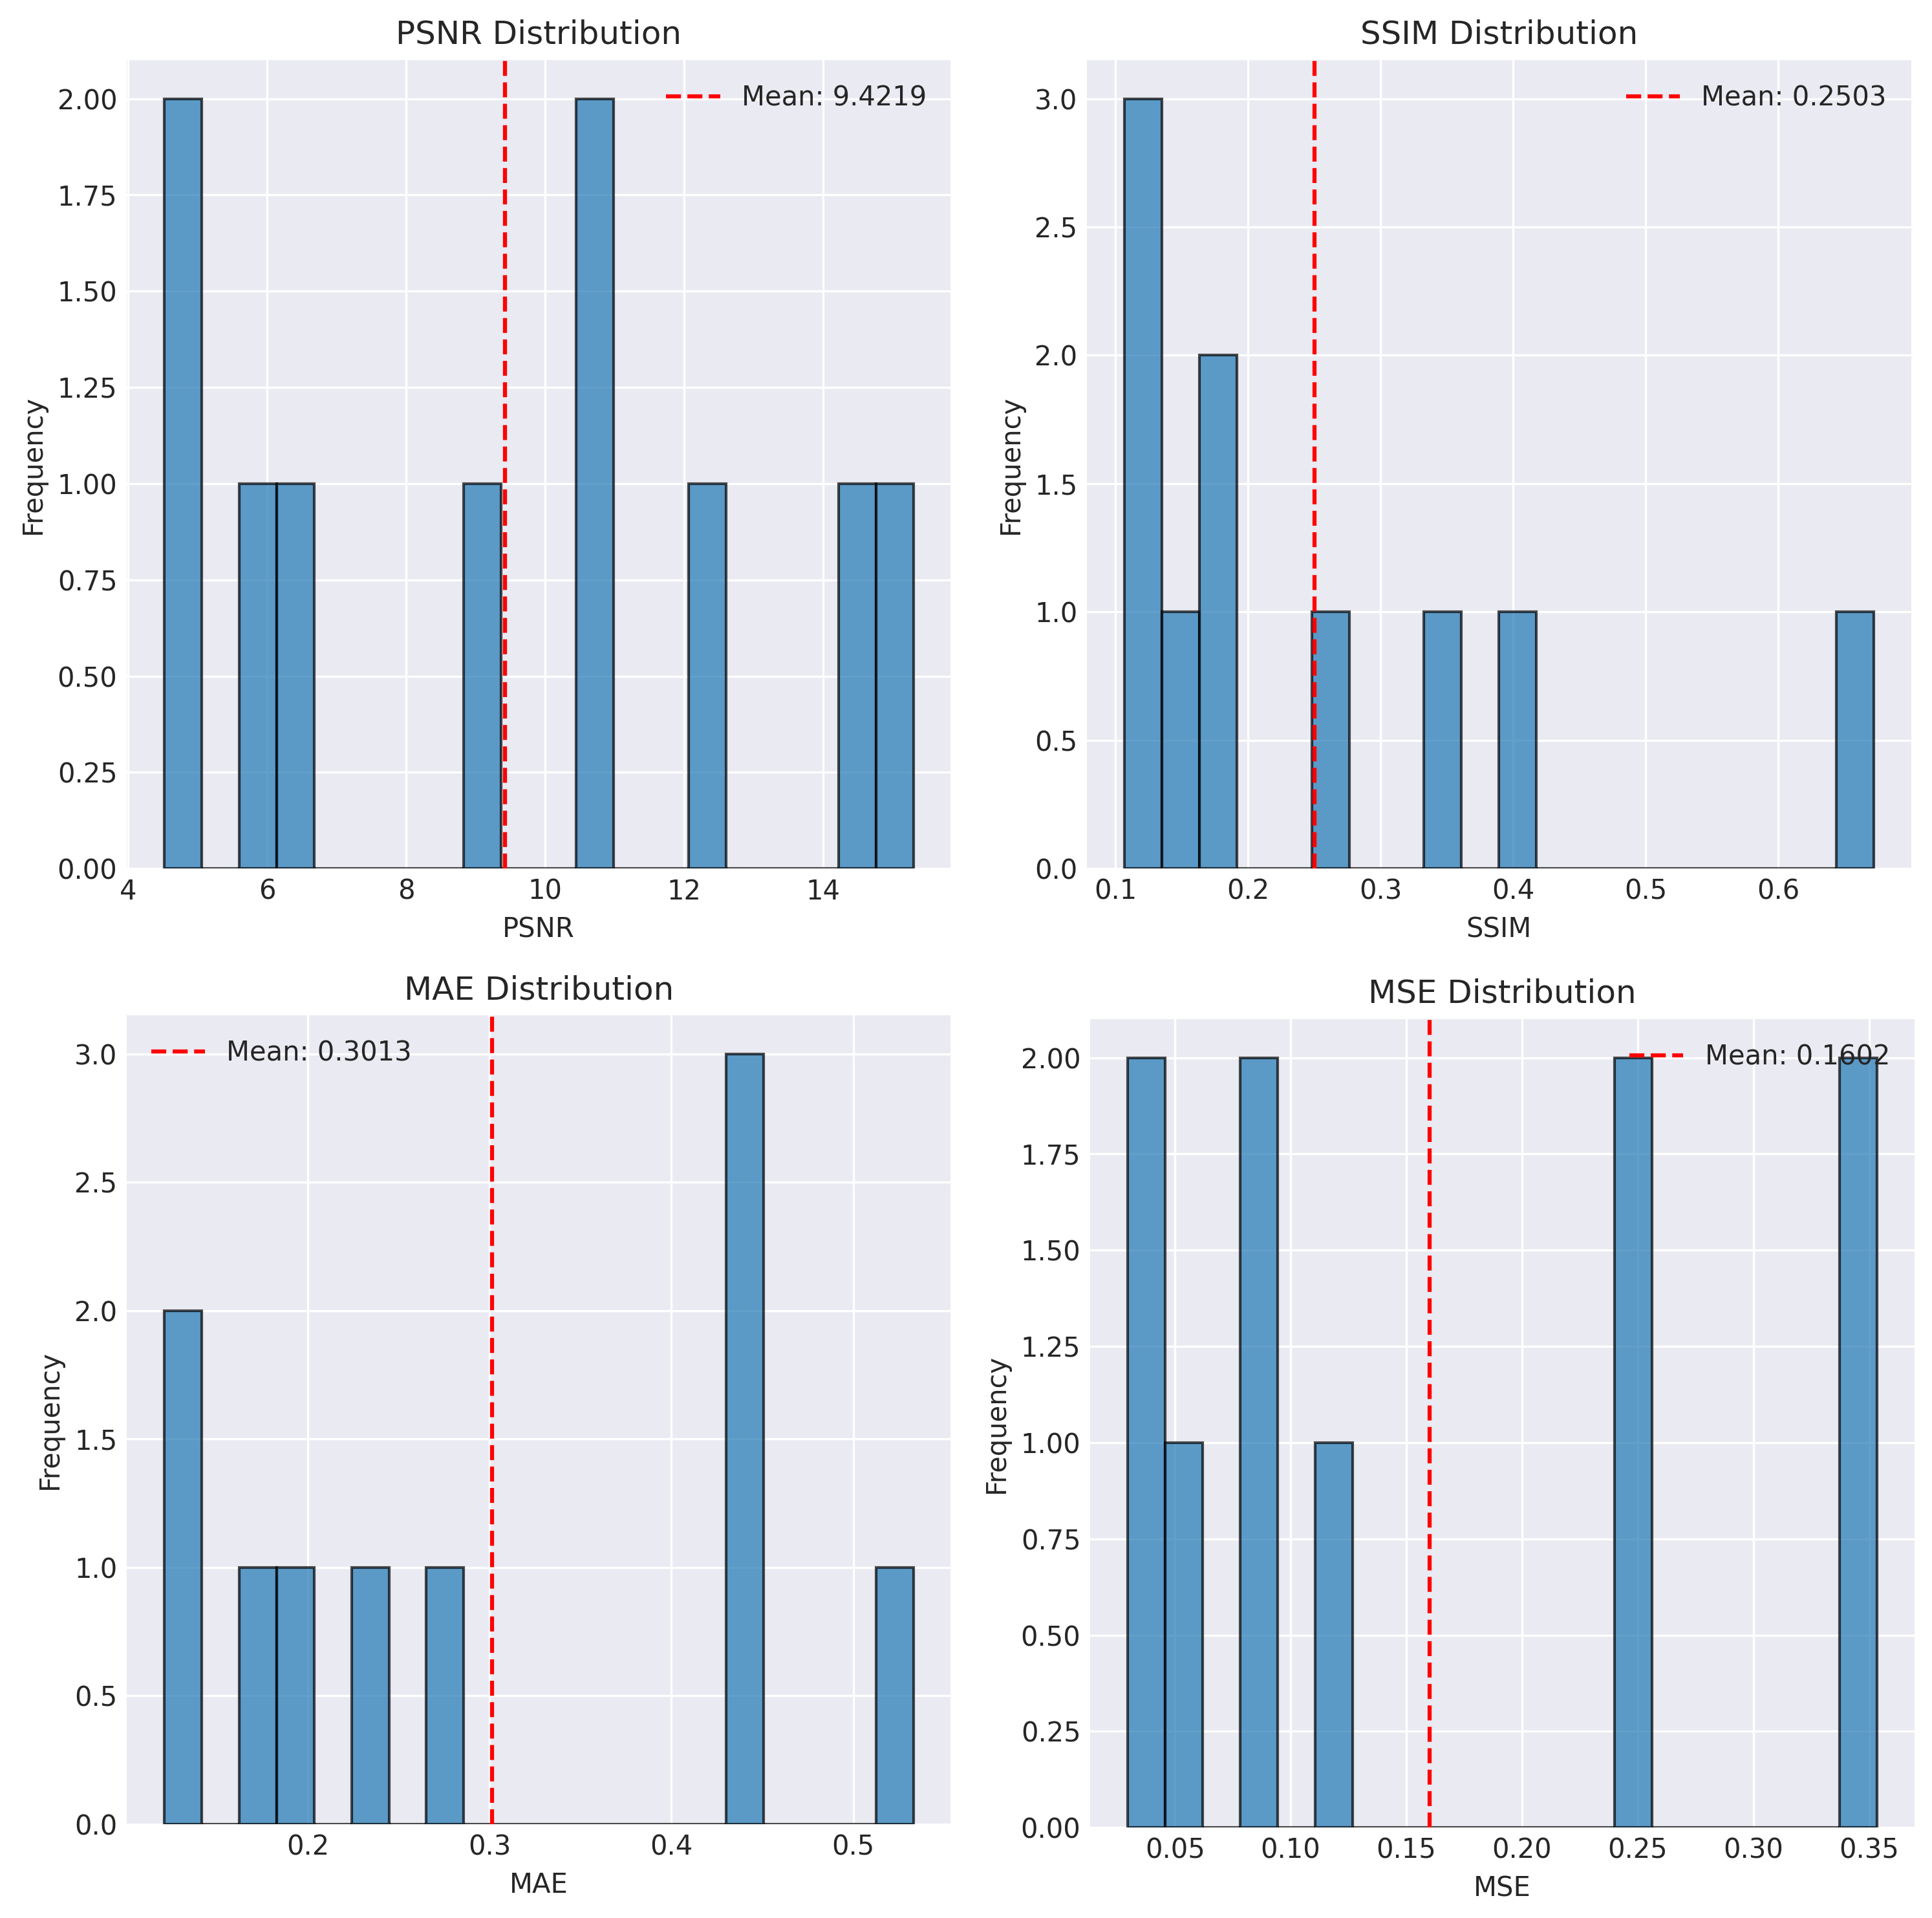
\includegraphics[width=0.8\textwidth]{metrics.png}
    \caption{Visualization of evaluation metrics distribution across test samples}
    \label{fig:metrics}
\end{figure}

\subsection{Limitations and Future Work}

\subsubsection{Current Limitations}
\begin{itemize}
    \item \textbf{Limited Dataset Size}: Evaluation on only 10 samples limits the statistical significance of results
    \item \textbf{Seasonal Variations}: Some seasonal contexts may be underrepresented in the training data
\end{itemize}

\subsubsection{Future Improvements}
\begin{itemize}
    \item \textbf{Expanded Evaluation}: Conduct evaluation on larger, more diverse test sets
    \item \textbf{Perceptual Metrics}: Incorporate perceptual quality metrics beyond pixel-level comparisons
    \item \textbf{Human Evaluation}: Include subjective assessment of visual quality and realism
\end{itemize}